\section {Aplicación desarrollada\label{desarrollo}}

Este capítulo tratará de hacer entender al lector el trabajo que se ha realizado y como funciona. Para ello, mostraremos los pasos que hemos seguido para montar cada una de las herramientas sobre la arquitectura seleccionada. 

\subsection {Hardware utilizado\label{hardware}}

La máquina que se ha usado para el desarrollo de este trabajo ha sido mi ordenador portátil por motivos de disponibilidad. Dicha máquina es un MSI GP60 2PE Leopard con las siguientes características:\par
\begin{itemize}
	\item MSI GP60 2PE Leopard
	\begin{itemize}
		\item Disco duro:
		\begin{itemize}
			\item SSD mSATA de 250 GB
			\item HDD SATA de 750GB
		\end{itemize}
		\item RAM: 16 GB
		\item Procesador: Intel Core i7-4710HQ
		\item Tarjeta gráfica: NVIDIA GeForce 840M
		\item Sistema operativo: Lubuntu 16.04
		\item Propietario: Rubén Garrido
	\end{itemize}
	\item Disco duro externo WD Elements Basic Storage:
	\begin{itemize}
			\item Capacidad 2 TB
			\item Formateado en ext4
			\item Propietario: Rubén Garrido
	\end{itemize}
\end{itemize}

\subsection {Datos obtenidos y preprocesado\label{datos}}

Para realizar las pruebas se han obtenido datos de diferentes fuentes. Por una parte, Movildata nos ha ofrecido los datos anonimizados de varios vehículos obtenidos durante tres días, en concreto, durante los días 28, 29 y 30 de Mayo. Dichos datos se almacenan en un JSON de 1,83 GB en el siguiente formato:\par

\begin{lstlisting}[frame=single]  
{
  {
	"_id": {
		     "$oid": "IDENTIFICADOR DE OBJETO"
	       },
	"metaData": [
		{
		  "keyName": "Type",
		  "units": "VehicleType",
		  "unitType": "string"
		}
	],
	"reports": [
		{
		   "identity": {
		   "sensorId": "IDENTIFICACION DIARIA QUE SE LE DA 
		                 AL VEHICULO"
		},
		  "measurements": [
		     {
		         "location": {
		                       "coordinates": [
		                                        LONGITUD, 
		                                        LATITUD, 
		                                        ALTURA
		                                      ], 
		                       "heading": "166",
		                       "temp": "TEMPERATURA",
		                       "speed": "VELOCIDAD",
		                       "speedmetric":"METRICA PARA 
		                                      LA VELOCIDAD"
		                     },
		          "observationTime": "FECHA",
                  "Type": "TIPO DE VEHICULO (camion, coche o bus)"
		        }
		  ]
		},
		....]
  }
}
\end{lstlisting}


Aquí podemos ver un ejemplo:\par

\begin{lstlisting}[frame=single]  
{
      "_id":   {
            "$oid":   "5afa9ec2d815bd6e3c12d0cf"
      },
      "metaData":   [
            {
                  "keyName":   "Type",
                  "units":   "VehicleType",
                  "unitType":   "string"
            }
      ],
      "reports":   [
            {
                  "identity":   {
                        "sensorId":   "651513"
                  },
                  "measurements":   [
                        {
                              "location":   {
                                    "coordinates":   [
                                          -1.317187,
                                          40.648389,
                                          994
                                    ],
                                    "heading":   "166",
                                    "temp":   "No",
                                    "speed":   "88",
                                    "speedmetric":
                                        "KilometersPerHour"
                              },
                              "observationTime":
                                    "2018-05-15T08:45:51.0000000Z",
                              "Type":   "truck"
                        }
                  ]
            },
     ....
      ]
}

\end{lstlisting}

Dado el formato de estos datos hemos tenido que preprocesarlos con Spark para obtener un fichero CSV equivalente, en el que cada trama se almacene en una sola línea. Esto se ha realizado para facilitar la simulación del envío de las tramas de los vehículos.\par

Una vez obtenido esto, para simular los usuarios, he creado 180 usuarios y he dividido, con una distribución aleatoria, los vehículos con los usuarios que hemos creado. De esta forma, simularemos la cantidad de vehículos que tienen los clientes reales de una empresa de este tipo, donde cada empresa tiene una cantidad determinada, según su necesidad. Esta distribución podemos verla en la figura \ref{userGraf}.\par

\begin{figure}[htp]
\centering
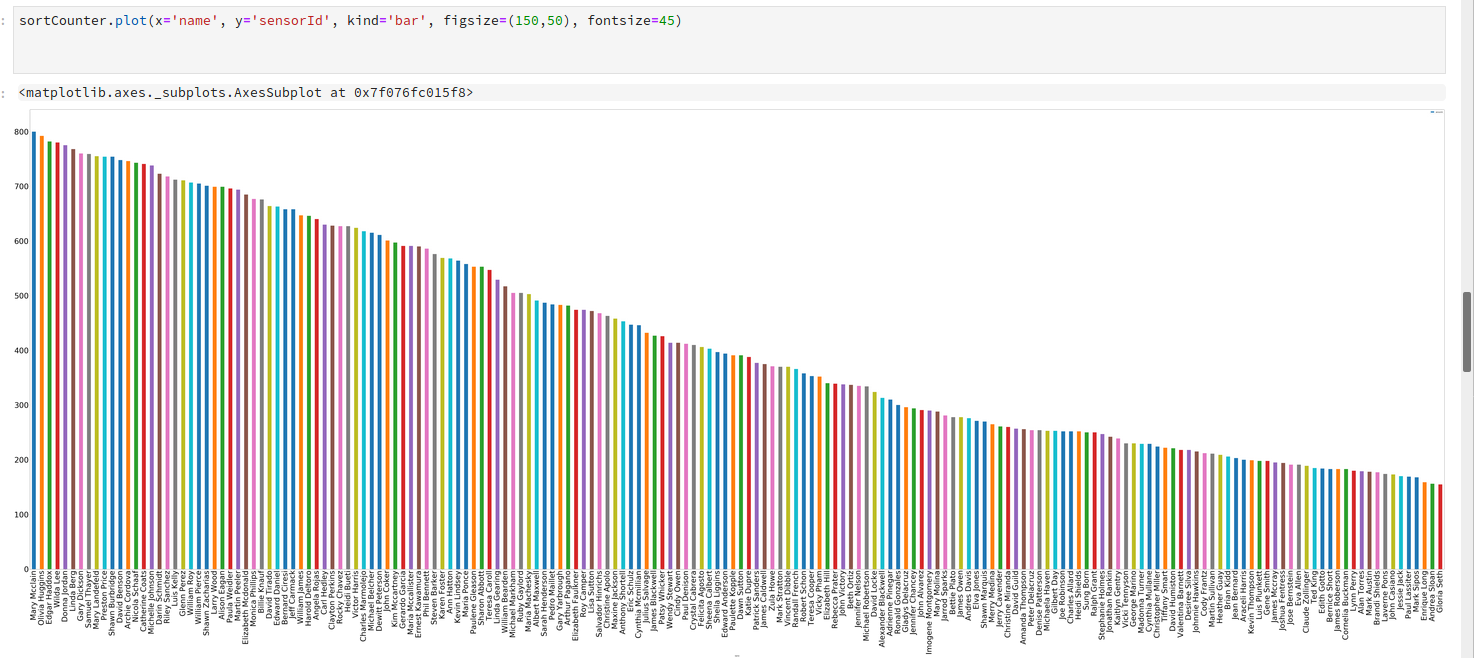
\includegraphics[scale=0.3]{Imagenes/graf1.png}
\caption{Cantidad de vehiculos para cada usuario.}
\label{userGraf}
\end{figure}

A partir de esto, crearemos dos CSV que almacenaremos en Hadoop, en la que aparezcan los nombres de los usuarios y la asociación de los vehículos con los usuarios. Con esto obtenemos 876 vehículos en el usuario que más vehículos y 168 en el que menos.\par
Por último, con los datos cedidos por Movildata, hemos obtenido dos gráficas que nos mostrarán la frecuencia de los datos cada 60 segundos y cada segundo en un día concreto. Esto lo podemos ver en las siguientes figuras (\ref{graf60sec} y \ref{graf1sec}), en las que vemos como el máximo número de tramas en un minuto es de 8000 y el máximo de tramas durante 1 segundo es de 250.\par

\begin{figure}[htp]
\centering
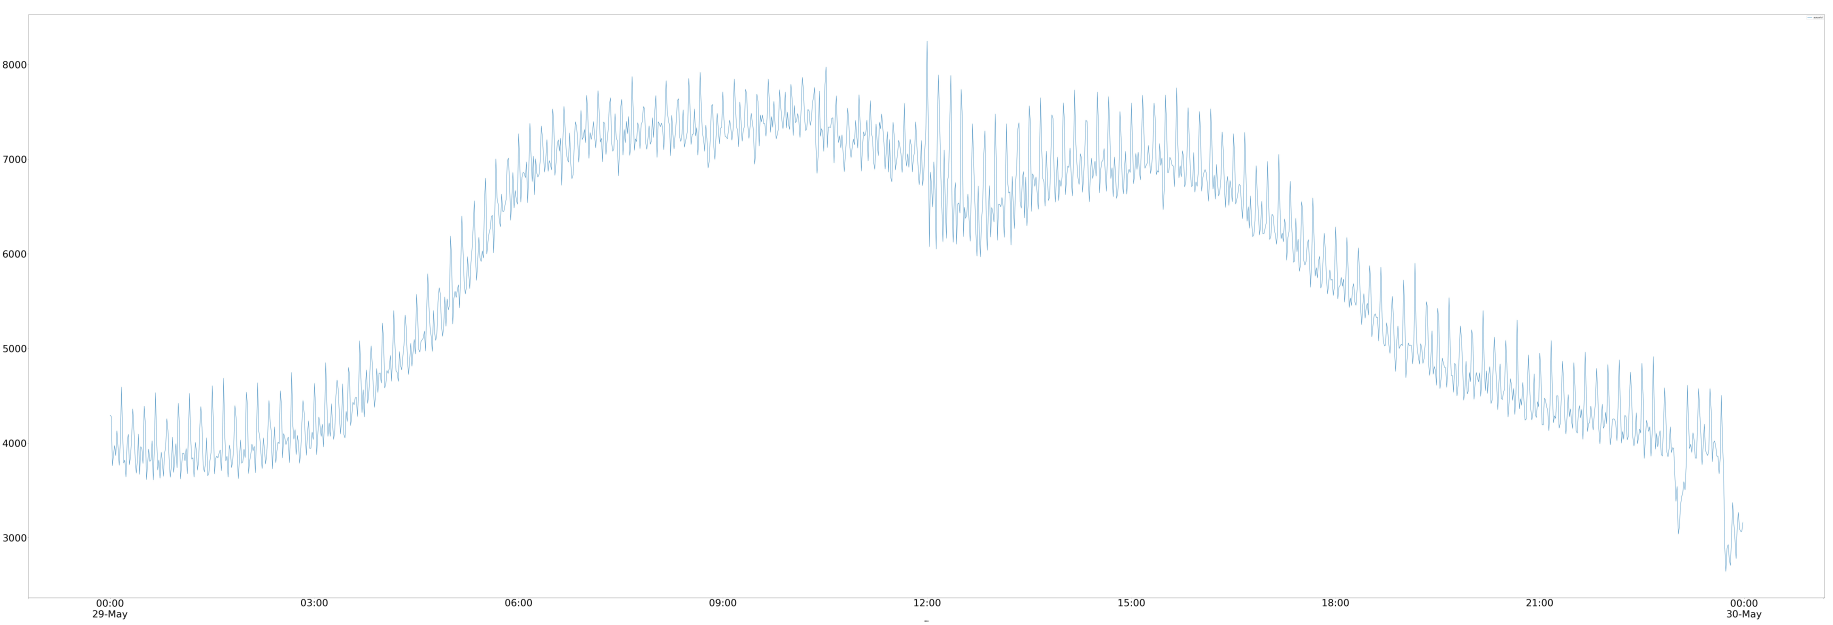
\includegraphics[scale=0.26]{Imagenes/graf2.png}
\caption{Frecuencia de las tramas durante un día cada 60 segundos.}
\label{graf60sec}
\end{figure}

\begin{figure}[htp]
\centering
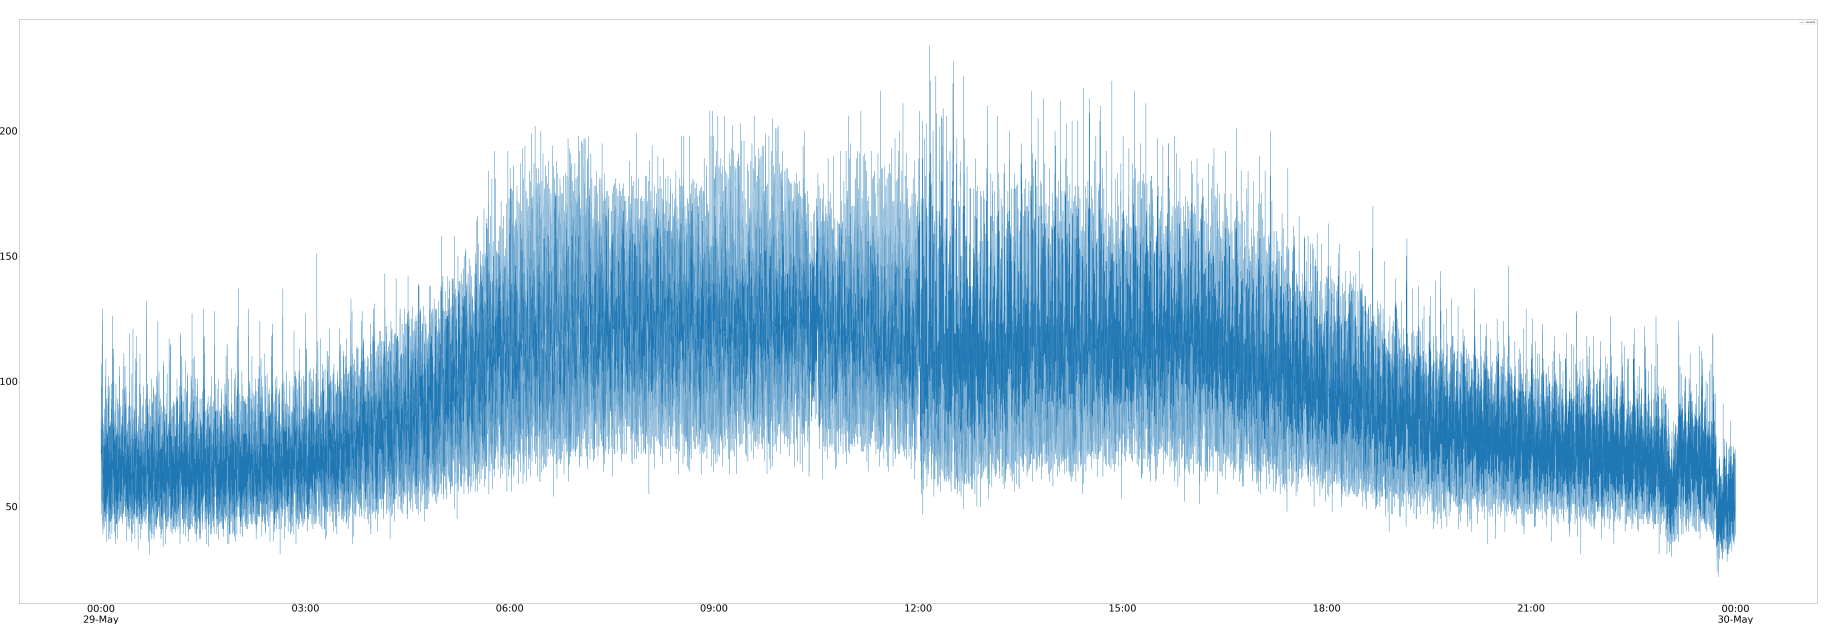
\includegraphics[scale=0.26]{Imagenes/graf3.png}
\caption{ Frecuencia de las tramas durante un día cada segundo.}
\label{graf1sec}
\end{figure}

Por otro lado, hemos obtenido de la DGT los puntos negros de España en 2014, que es el último documento público actualizado que hemos encontrado. Dicho documento es un excel con varias hojas, una por cada provincia o región de España, y en cada hoja se detalla la dirección del punto donde se han eventuado accidentes y se consideran puntos negros. Debido a la dificultad del formato y que no tenemos los puntos geográficos, se ha realizado un preprocesamiento para obtener un CSV más fácil de procesar por los servicios que vamos a crear. Dicho preprocesamiento aplana el excel en un solo csv y, además, obtiene los puntos geográficos a través del API de Google Maps usando la función de georreferenciación inversa.
Finalmente, se han obtenido los datos de los mapas de OSM, concretamente se han obtenido los datos del mapa de España en un fichero .osm para, posteriormente, poder procesarlo e insertarlo en la base de datos seleccionada.

\subsection{Detalles de implementación\label{implementacion}}

Dedicaremos esta sección a explicar en detalle el desarrollo realizado. Dicho esto comenzaremos explicando cómo se va a ver la arquitectura a grandes rasgos hasta llegar al detalle de implementación de cada herramienta.

\subsubsection{Diseño de la arquitectura con las herramientas seleccionadas\label{disenio}}

En cuanto a la arquitectura desarrollada, planificamos una estructura como la que se muestra en la figura \ref{lmdarq1}. En esta arquitectura encontramos los datos ofrecidos por Movildata como emisor de los datos, los cuales llegarán a una cola de Kafka. Dichos datos serán recogidos por Hadoop para almacenarlos en bruto en HDFS. Por otro lado, Spark recogerá los datos de la cola para realizar el procesamiento en tiempo real, es decir, para asociarlos con el usuario y detectar anomalías. Tras realizar el procesamiento, Spark insertará en otra cola de Kafka los datos, los cuales serán leídos por Logstash para insertarlos en Elasticsearch. Una vez insertados en Elasticsearch seremos capaces de mostrarlos en tiempo real a través de Kibana, donde configuraremos diferentes gráficos y dashboard.\par

\begin{figure}[htp]
\centering
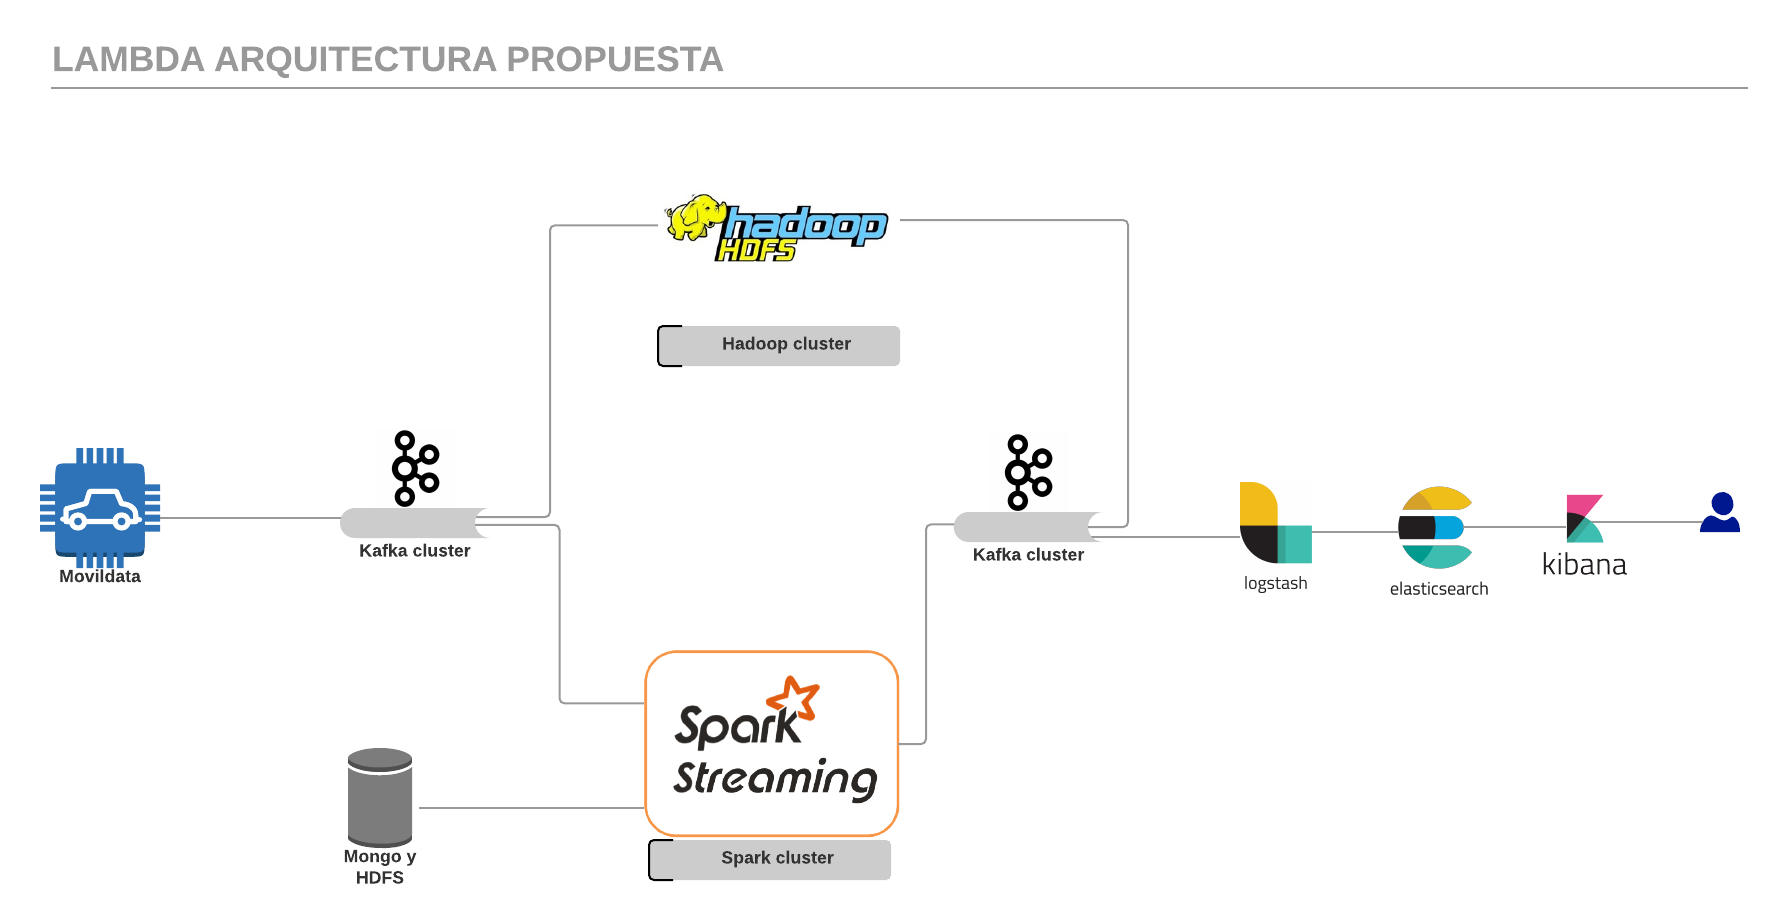
\includegraphics[scale=0.26]{Imagenes/arqProp1.png}
\caption{Lambda arquitectura propuesta.}
\label{lmdarq1}
\end{figure}

Para realizar esto, lo primero que se ha realizado es configurar los diferentes Dockerfiles para establecer las imagenes de nuestros container. Para ello, usaremos la herencia que nos proporciona Docker y crearemos un esquema como el que aparece en la figura \ref{lmdarq2}. Como padre tendremos una imagen de Ubuntu que contendrá todas las librerías comunes para todos. Por consiguiente, crearemos una imagen padre para Hadoop, Zookeeper, Kafka, Spark, las tecnologías de Elastic y MongoDB, teniendo en cuenta que Zookeeper estará por encima de Kafka, ya que es necesario para que Kafka funcione. A partir de este diseño, comenzaremos a explicar los entresijos de cada una de estas imágenes.

\begin{figure}[htp]
\centering
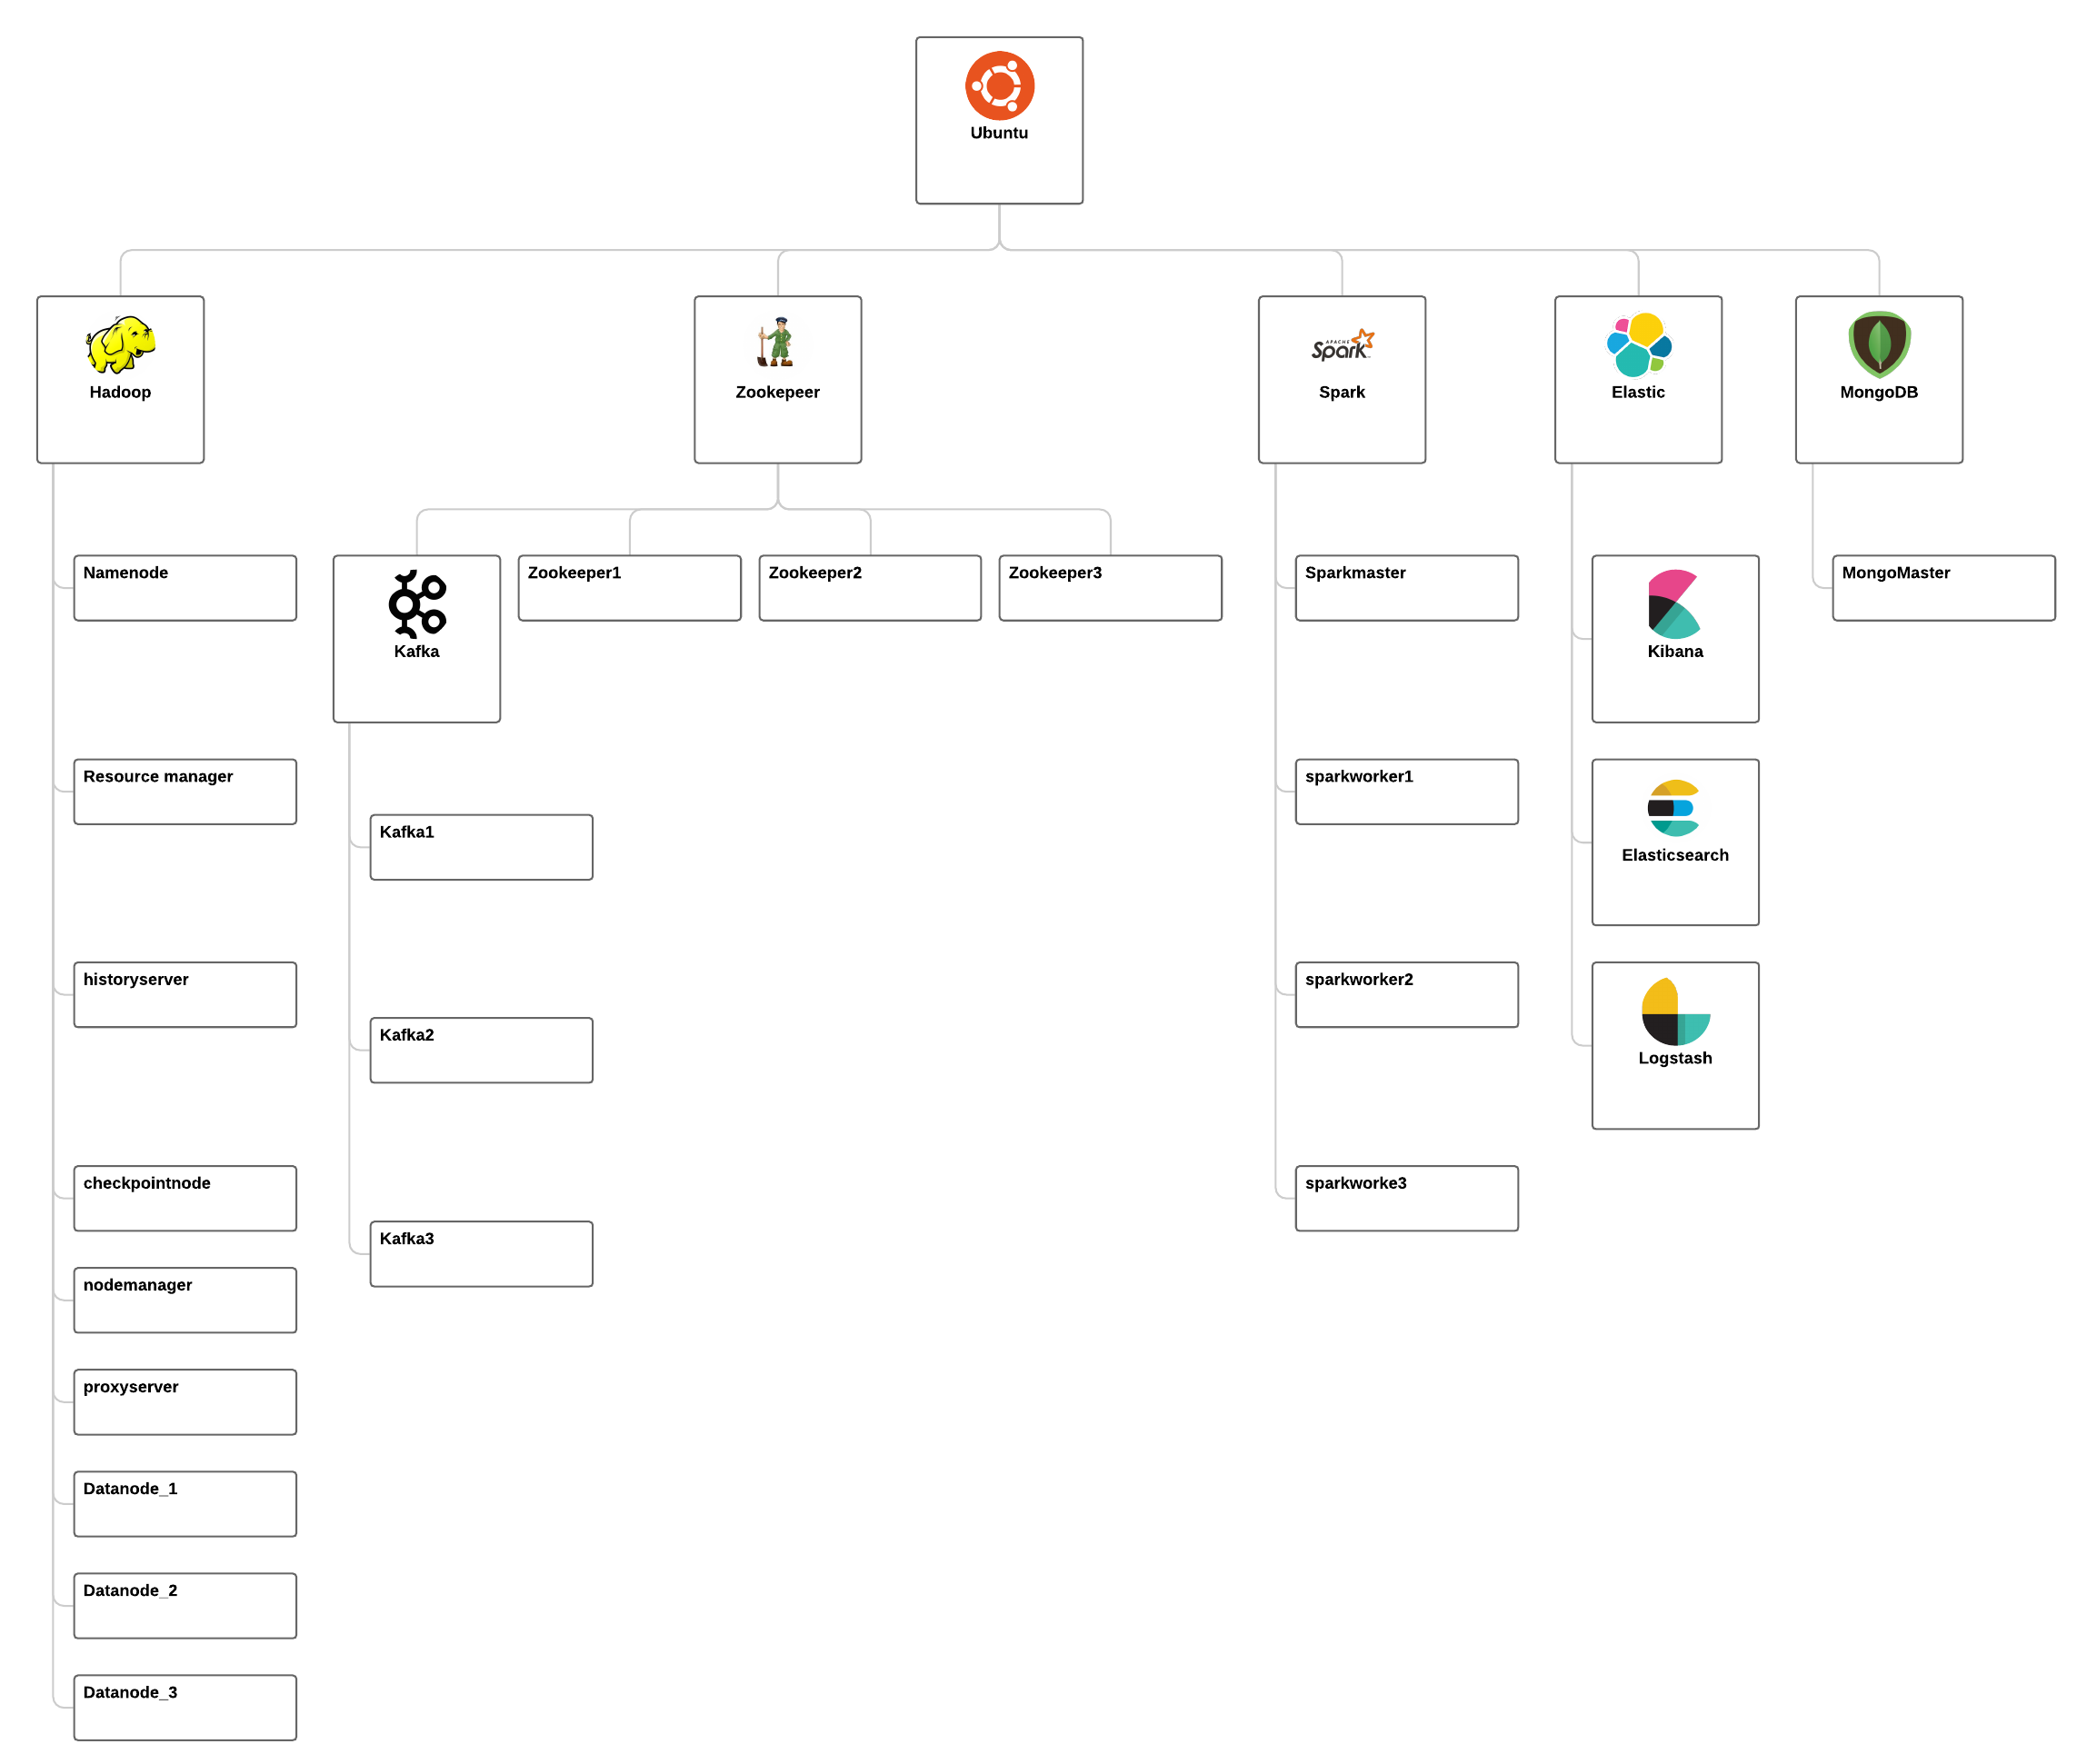
\includegraphics[scale=0.20]{Imagenes/arqProp2.png}
\caption{Esquema jerárquico docker.}
\label{lmdarq2}
\end{figure}

\subsubsection{Montaje de la imagen de Ubuntu\label{montUbuntu}}

Para crear esta imagen, hemos usado la imagen oficial de Ubuntu que encontramos en Docker Hub. A partir de esta imagen, hemos instalado SSH para tener interconectadas todas las máquinas que creemos. Para que la conexión sea segura y no necesitemos acceder a través de contraseña, hemos generado un certificado RSA y hemos establecido en el fichero de configuración de SSH "ssh\_config", que se encuentra en el directorio "/etc/ssh/", el parámetro  "SET StrictHostKeyChecking" a  "no" para que no pregunte si desea conectarse y se conecte automáticamente.\par

Para finalizar, hemos instalado en esta máquina Java 8, Scala 2.12 y Python 3. Java es necesario para que puedan ejecutarse Hadoop, Zookeeper y las herramientas de Elastic. Scala será necesario para Spark y Kafka. Por último, nuestros desarrollos se realizarán en Python 3. Dado que es un lenguaje muy fácil de usar no necesitamos compilar, esto hará que el desarrollo de esta prueba de concepto sea más ágil.\par

\subsubsection{Pasos a seguir para añadir aplicaciones sobre la imagen de Ubuntu\label{pasosUbuntu}}

En este subapartado, explicaremos los pasos a seguir para añadir aplicaciones y sea más fácil actualizarlas en un futuro, se debe seguir la siguiente estructura:

\begin{enumerate}

\item Se debe añadir un directorio, cuyo nombre sea el propósito de la aplicación, al directorio “/opt”. Un ejemplo de esto serían Hadoop, cuyo propósito es almacenar datos sobre su HDFS y procesarlos, por lo que entrará dentro de la categoría de base de datos y crearemos el directorio “/opt/bd”.

\item Sobre el directorio creado se debe descargar la aplicación con el nombre y la versión que le corresponde. Siguiendo el ejemplo anterior, para Hadoop, añadiremos el directorio de la aplicación como “/opt/bd/hadoop-3.1.0”.

\item En ese mismo directorio se debe crear un link al directorio de la aplicación con el nombre de la misma, de forma que, cuando queramos actualizar la aplicación, simplemente tendremos que cambiar el link del directorio.

\item Por último, como norma más importante, las variables de entorno de la aplicación deben apuntar al directorio creado como link y no al directorio creado en el paso 2 de la aplicación.

\end{enumerate}


Por otro lado, para configurar los ficheros donde las aplicaciones almacenarán los datos y los logs de las aplicaciones deberán seguir los siguientes pasos:

Se creará un directorio en “/var/data” en el caso de los datos de aplicación y un directorio en /var/log para el caso de los log con el nombre de la aplicación. En el caso de Hadoop, por ejemplo, sería     /var/data/hadoop en el caso de los datos y “/var/log/hadoop” en el caso de los logs.
\begin{enumerate}

\item Dadas las características de Docker, para añadir la persistencia, dichos directorios se deben establecer como volúmenes o como enlaces a directorios propios del sistema. En nuestro caso, estableceremos enlaces a los directorios del sistema y los enlazaremos a un directorio que seguirá la siguiente nomenclatura “nombre de la aplicación” + “\_resources”. Siguiendo con el ejemplo de Hadoop, crearemos un directorio cuyo nombre será     “hadoop\_resources”.         

\item Dado que podemos tener varios servicios por aplicación, tendremos que crear, dentro de este directorio, otro directorio con el nombre del servicio. Siguiendo el ejemplo de Hadoop y haciendo referencia al servicio datanode, crearemos el directorio “hadoop\_resources/datanode/”

\item Para terminar, dentro de este directorio debemos crear los directorios data y log que serán los que realmente enlazarán con el directorio que corresponde a los del paso 1. Para seguir con el ejemplo, tendremos que crear los directorios “./hadoop\_resources/datanode/ data” para los datos, y “./hadoop\_resources/datanode/log” para los logs. Esto lo podremos enlazar a través del comando correspondiente de Docker o en el fichero “docker-compose” que define cómo se lanzarán los servicios.

\end{enumerate}

Por último, decir que en cada una de las aplicaciones se debe definir un fichero Host que contendrá las rutas DNS que queramos añadir al fichero “/etc/hosts”. Al inicio, cada servicio se deben añadir estas rutas a dicho fichero. Los nombres que se establezcan únicamente pueden tener caracteres alfanuméricos debido a algunas incompatibilidades con algunas aplicaciones. Gracias a esto, los nombres de los servicios serán más amigables, por lo que será más sencillo acceder a los mismos.\par

\subsubsection {Montaje de las imágenes de Hadoop\label{montHadoop}}
Para la realización de este apartado, hemos usado Hadoop 3.1, aunque también hemos probado la versión 2.7, que es la que más se usa actualmente. Siendo así, ambas mantienen la misma estructura, a excepción de algunos parámetros de configuración que varían de una versión a otra o que quedan obsoletas. Las dos versiones están disponibles y funcionales tanto en GitHub como en Docker Hub. Dado que es una prueba de concepto, usaremos la versión superior por defecto, pudiendo comprobar de esta forma que el funcionamiento de la última versión es correcto y, cuando se desee integrar, podamos usar las últimas versiones de Hadoop.\par

Las imágenes de Hadoop constan de varias partes. Por un lado, encontraremos la configuración básica que dará lugar al cluster y por otro lado, las ejecuciones de los servicios en máquinas independientes como recomienda la filosofía de Docker. La imagen base consta de la instalación básica de Hadoop para el usuario “hdmaster”, que se almacenará en “/opt/bd/hadoop” (siguiendo los pasos explicados en la sección anterior), y el fichero de redirección DNS de todos los componentes del cluster. Además de esto, añadiremos las variables de entorno que Hadoop requiere para su ejecución: HADOOP\_HOME, HADOOP\_COMMON\_HOME, HADOOP\_HDFS\_HOME, HADOOP\_MAPRED\_HOME y HADOOP\_YARN\_HOME que apuntan al directorio de de instalación de Hadoop que hemos comentado y HADOOP\_CONF\_DIR y YARN\_CONF\_DIR que apuntan al directorio donde se encuentran los ficheros de configuración de Hadoop (“/opt/bd/hadoop/etc/hadoop”). Por último, respecto a la configuración que viene por defecto en Hadoop, hemos modificado los siguientes ficheros de configuración:\par

\begin{itemize}
	\item core-site.xml
	\begin{itemize}
		\item Definimos la referencia al namenode como “hdfs://namenode:9000”.
		\item Usuario estático por defecto como “hdfs” .
		\item El directorio temporal en “/var/tmp” ya que no necesitamos que sea persistente.
	\end{itemize}
	
	\item hadoop-env.sh
	\begin{itemize}
		\item Definimos la ruta a Java a JAVA\_HOME.
	\end{itemize}
	
	\item hdfs-site.xml
	\begin{itemize}
		\item Establecemos el factor de replicación de bloques a 2. Por defecto está a 3, que son demasiados para este proyecto.
		\item El tamaño de bloque se establecerá a 64 megas. Por defecto está a 256 megas, que es demasiado grande para nuestro propósito.
		\item Establecemos la interfaz web para que esté disponible.
		\item Estableceremos el directorio donde el namenode guardará los metadatos a “/var/data/hadoop/hdfs/nn”.
		\item Establecemos el directorio donde el nodo checkpoint guarda los checkpoint y los los edits temporales a “/var/data/hadoop/hdfs/cpn”.
		\item Establecemos el directorio donde los datanodes guardan los datos a “/var/data/hadoop/hdfs/dn”.
		\item Establecemos la interfaz de acceso al datanode a “namenode:50070”.
		\item Establecemos la interfaz del nodo checkpoint a “checkpointnode:50090”.
		\item Establecemos que el usuario y grupo hdfs, que será el que aparezca en la interfaz web, tenga permisos para subir y borrar ficheros del HDFS.
	\end{itemize}
	
	\item mapred-site.xml
	\begin{itemize}
		\item Definimos que usaremos el framework yarn, que será el que realiza el MapReduce.
		\item Definimos el JobHistory a historyserver:10020 y la interfaz web a historyserver:19888.
		\item Establecemos el uso máximo de memoria a 1GB tanto para Map como para Reduce.*
	\end{itemize}
	
	\item yarn-site.xml
	\begin{itemize}
		\item Establecemos el nombre del resourcemanager y la dirección a “resourcemanager:8032”.
		\item Establecemos los logs de aplicaciones sobre el historyserver.
		\item Establecemos el sistema de map como ShuffleHandler.
		\item Establecemos el directorio de logs a “var/log/hadoop/yarn”
		\item Establecemos el uso de cores a 4 por nodo.*
		\item Establecemos el máximo de uso de memoria por contenedor a 4GB.*
		\item Establecemos el ratio de memoria física y virtual a 4.
		\item Establecemos el mínimo de memoria reservada a 1GB.*
		\item Establecemos el proxy a “proxyserver:50070” 
	\end{itemize}
	
	\item workers
	\begin{itemize}
		\item Dicho fichero tiene los nombres de los nodos que se desean establecer como “workers” o trabajadores. Aquí, estableceremos como workers a los nodos  nodemanager, el namenode, el datanode1, el datanode2 y el datanode3. Posteriormente, dichos nodos serán establecidos como workers a través del nodemanager.
	\end{itemize}
\end{itemize}

Una vez hecho esto, definiremos los diferentes servicios de Hadoop especificados en la sección 2.5. Para ello, crearemos diferentes imágenes que lanzarán un shell llamado “run.sh” que simplemente se asegurará de que los puertos que necesita cada uno esté abierto y lance su servicios, a excepción del namenode. El servicio de namenode se encargará de montar el sistema de ficheros HDFS y, para que en posteriores ejecuciones no se vuelva a lanzar, en su directorio persistente guardará que ya está creado.\par

Para terminar con la configuración, crearemos un fichero docker-compose.yml con el que podemos probar el cluster compuesto por tres datanodes.\par

Por último, decir que la versión 2.7 de Hadoop, al realizar los diferentes test que vienen con la aplicación, consume más RAM que la versión 3.1. El haber realizado las pruebas con Hadoop 2.7 también es porque es la versión oficial compatible tanto para Spark como para Flink (solo usaremos Flink para comprobar que Spark es una herramienta que podemos reemplazar fácilmente) y, tras haber comprobado las diferencias, hemos llegado a la conclusión de que la única parte de Hadoop 3.1 que no es compatible con estos es la de asignar la memoria y los cores que usa de forma dinámica. Dado esto, hemos establecido en los ficheros de configuración la asignación de memoria y los cores de forma fija (aparecen con un asterisco).\par


\subsubsection {Montaje de las imágenes de Zookeeper y Kafka\label{montKafka}}
Apache Zookeeper es un orquestador que nos ayudará a volver a seleccionar líderes en los cluster de Apache Kafka y, posteriormente, de Apache Spark, por lo que lo añadiremos en la ruta “/opt/orchestrator”. Para configurar esta herramienta, crearemos un cluster de Zookeeper que se dedique a esto. Para ello, en el fichero de configuración “zoo.cfg” estableceremos las direcciones de los nodos del cluster y le especificaremos que trabajará como tal.\par

En cuanto a Apache Kafka, dado que es un gestor de colas, lo añadiremos en la ruta “/opt/queuesmanager”. En cuanto a la configuración, se encuentra en el fichero “server.properties”, en el cual añadiremos las direcciones del cluster de Zookeeper. Por otro lado, dado que hay que asignarle un identificador a cada uno de los nodos, asignaremos una forma de lanzarlo dinámicamente. Para ello, estableceremos con “@id” como marca para posteriormente establecer el identificador. Aprovechando esta tarea, estableceremos el nombre del host de la misma forma como “@hostname”.  Por último, asignaremos el número de particiones por defecto a 1, al igual que el factor de replicación.\par

Para lanzar los diferentes contenedores de Kafka, lanzaremos un shell que modifique el fichero de configuración estableciendo los valores que haya que asignar y, posteriormente, lance el proceso de Kafka.\par


\subsubsection {Montaje de las imágenes de Spark\label{montSpark}}

Para montar la imagen de Apache Spark, añadiremos la aplicación en “/opt/bd/streaming”, debido a que se conectará con la base de datos para realizar el streaming. Por otro lado, estableceremos en el fichero “spark-defaults.conf” la siguiente configuración:\par
\begin{itemize}
	\item Asignamos, por defecto, user “yarn” es decir, el cluster de Hadoop.
	\item Establecemos que reserve como máximo de memoria 512MB, tanto para el yarn como para el cluster de Spark.
	\item Establecemos los logs.
	\item Asignamos los ficheros de logs si usa el yarn en el directorio “hdfs://namenode:9000/user/ hdmaster/spark-logs”.
	\item Establecemos el history server de Spark.
	\item Establecemos el puerto para la web de Spark a “18080”.
	\item Seleccionamos dónde se albergan las librerías de Spark en el hdfs a “hdfs://namenode:9000/ user/hdmaster/spark-archives.zip”
	\item Le confirmamos que la replicación de bloques del yarn está a 2.
	\item Le especificamos dónde está el cluster de Hadoop y con los puertos por los que se debe comunicar con: “hdfs://namenode:9000, hdfs://datanode1:9866, hdfs://datanode2:9866, hdfs://datanode3:9866”
	\item Establecemos el acceso a datos de HDFS a “hdfs://namenode:9000”
	\item Especificamos que la forma de recuperación, en caso de caÍdas, para seleccionar un nuevo líder, lo haremos con Zookeeper. Esta integración se hará automática añadiendo las direcciones del cluster de Zookeeper “zoo1:2181, zoo2:2181, zoo3:2181”
\end{itemize}

Por otro lado, añadiremos como esclavos en el fichero “slaves”, que serán los procesos de Spark que ejecutarán trabajos, a los nodos sparkmaster, sparkworker1, sparkworker2 y sparkworker3, para el caso que queramos ejecutar el cluster de Spark.\par

Para terminar con la configuración de la imagen base de Spark, decir que para poder usar pyspark con Python 3, hemos establecido la variable de entorno “PYSPARK\_PYTHON” a “python3”, ya que, de no ser así, usará por defecto Python2. Por otra parte, también hemos establecido que el código de Python será introducido con codificación UTF-8, de manera que minimizaremos los problemas con caracteres españoles. Para ello, estableceremos la variable de entorno “PYTHONIOENCODING” a “UTF-8”. \par
Con esta configuración, seleccionará por defecto los workers de Hadoop para ejecutar los trabajos. Hadoop debe contener las librerías de Spark para poder hacer uso de ellas, por lo que será necesario que estén introducidas en la ruta del HDFS especificadas. Para esto, cuando definamos el nodo spark-master, llevará a cabo su ejecución de la siguiente forma:\par
\begin{enumerate}
	\item Cuando esté lanzado el contenedor por primera vez, esperará 14 segundos, dado que no hay forma de saber si el HDFS está montado.
	\item Cuando hayan pasado los 14 segundos correspondientes, tendrá que comprobar de un fichero que esté guardado de forma persistente, si se han añadido ya las librerías de Spark al HDFS. Esto lo sabremos si se ha ejecutado anteriormente el script que las añade.
	\item Una vez hecho esto, los slaves y el history-server de Spark estarán esperando a que el spark-master lance sus demonios.
\end{enumerate}
Para cumplir con los requisitos, hemos hecho también pruebas con Apache Flink, comprobando que podemos cambiar la herramienta si en algún momento se requiere valorando esta alternativa cuando esté más madura en el mercado. Dado que usamos Kafka, también hemos comprobado que podemos usar ambas herramientas a la vez sin ningún problema, ya que pueden existir varios suscriptores en las colas.



\subsubsection {Montaje de las imágenes Elastic\label{montElastic}}

Para el montaje del Stack de Elastic introduciremos Elasticsearch, Logstash y Kibana en /opt/bd, en la imagen base. En la configuración de Elasticsearch, en el fichero “elasticserhc.yml”, estableceremos el nombre del cluster a “elastic-cluster”, como nombre descriptivo lo estableceremos a “elastic-1-master”, la ruta del host a “elasticserach” (está en la ruta del DNS), el puerto a 9200 y la ruta a datos y al log como se establece en el apartado \ref{pasosUbuntu}. Por la parte de Logstash, estableceremos en el fichero “logstash.yml”, el nombre del nodo a logstash-1, que puede usar dos núcleos de la CPU y las rutas de datos y log como se establece en el apartado \ref{pasosUbuntu} Por último, para configurar Kibana ejecutaremos en el fichero “kibana.yml” la ruta al host como Kibana (está en la ruta del DNS), en el puerto 5601, la ruta a Elasticsearch a "http://elasticsearch:9200" y el fichero de log como se establece en el apartado \ref{pasosUbuntu}.\par

Para hacer uso de las aplicaciones de una forma más fácil, estableceremos las variables de entorno ES\_HOME, que contendrá la ruta a Elasticsearch, ES\_PATH\_CONF, que contiene la ruta al fichero de configuración a Elasticsearch, LOGSTASH\_HOME, que contendrá la ruta a Logstash, y KIBANA\_HOME, que contendrá la ruta de Kibana.\par
Para lanzar los servicios, crearemos una imagen para Elasticsearch, que lanzará Elasticsearch, la de Kibana lanzará Kibana y la de Logstash no lanzará nada para poder realizar las diferentes pruebas.\par

\subsubsection {Montaje de las imágenes de MongoDB en integración de OSM\label{montMongo}}
Para montar Mongo DB, crearemos una imagen en la que añadiremos el repositorio oficial que contiene la versión 3.6 de MongoDB y lo instalamos con “apt-get”, por lo que no seguirá la configuración del apartado \ref{pasosUbuntu}. En el fichero mongodb.conf asignaremos la ruta a los ficheros de datos y logs como se especifica en el apartado \ref{pasosUbuntu}, la ruta como mongomaster y el puerto 27017. Por último, crearemos la imagen que lanza MongoDB.\par

Para integrar los datos de OSM, usaremos esta misma imagen añadiendo el mapa de España. Para subir los datos nos basaremos en un proyecto de GitHub que recomiendan en la página oficial de OSM. Dicho proyecto contiene unos scripts de Python que hemos actualizado a Python 3 para que sea compatible con nuestros proyectos. Una vez hecho esto, usando estos los scripts, hemos usado el fichero especificado en el apartado \ref{datos} del mapa de España y lo hemos subido a nuestra base de datos de MongoDB. Dado que los datos se almacenan en “/var/data/mongodb”, podremos transportarlos entre los container que queramos.\par

Dado esto, crearemos una API web para poder consultar la información de un punto, de forma que no tengamos que abrir las conexiones a la base de datos cada vez que se realiza una consulta. Se ha de tener en cuenta esto, ya que, si trabajamos con programas que se ejecutan en un cluster, cada una de las máquinas del cluster ejecutará diferentes partes del código y no podemos asegurar que una sola máquina realice la ejecución de las consultas a la base de datos. Dado esto, crearemos dicha API, con Python y la librería werkzeug, con la que podremos consultar un punto geográfico. Esta API nos devolverá la información de la carretera de la base de datos que más se aproxime al punto que pidamos, en un radio de 1,11 km. El código se puede ver en el anexo 9.1, y podremos realizar consultas a través de la url “http://mongomaster:5000/getway/<latitud>/<longitud>” que nos devolverá un JSON con los datos que se encuentran en la base de datos.\par

\subsubsection {Integración de los datos de pruebas \label{integracion}}    
     
Para que los datos se introduzcan en Kafka simularemos con un script de Python los mensajes que se recibirán de los vehículos. Este script introducirá un JSON por cada trama en el topic “streamKafka” de Kafka.\par

Tras esto, haremos el preprocesamiento de Spark Streaming. Para ello, debemos introducir, en el HDFS, los CSV creados de los usuarios y la asociación de los vehículos para, posteriormente, cargarlos. Por otro lado, tendremos que integrar los datos de los puntos negros, por lo que subiremos también el CSV al HDFS.\par

Una vez subidos los datos, probaremos Spark Streaming y SparkSQL Streaming para ver cómo se comportan. Esto lo encontraremos en el \textcolor{red}{ANEXO 9.3. y 9.4}. Dicho esto, comprobamos que los conectores a Kafka son diferentes al igual que la configuración de tiempo del microbatching, además de comportarse de forma distinta. En dichas pruebas, que consisten en recoger las tramas y asociar los vehículos con sus usuarios, comprobamos que Spark Streaming se comporta mejor que SparkSQL Streaming. Dado esto, seleccionamos Spark Streaming para realizar las pruebas. Por otro lado, para la asociación de los vehículos y los usuarios, probamos si funciona mejor con SparkSQL cambiando de contexto o con un rdd de Spark y comprobamos que SparkSQL funciona mejor, ya que, además de que es más fácil de usar, crea un batch con la concatenación de las diferentes aplicaciones que realizamos sobre los conjuntos de datos.\par

El script de Spark Streaming realizará lo siguiente:

\begin{itemize} 
	\item Cada 10 segundos se añade un trabajo a la cola de trabajos de Spark que se ejecutarán si el cluster no está ejecutando ningún otro proceso de esa misma cola.
	\item Cada uno de esos trabajos leerá de Kafka los 10 segundos que le corresponden indiferentemente de si corresponden en el tiempo o no. Esto es porque puede ser que algún trabajo se retrase, en ese caso, los trabajos retrasados se ejecutarán tras haber terminado el anterior.
	\item El proceso convertirá los JSON leídos de Kafka en una Dataframe de SparkSQL.
	\item Posteriormente, filtrará los datos erróneos, es decir, los que no son del día actual. En el caso de la simulación, los que no sean de los días que hemos recogido los datos.
	\item Se realizará los JOINs correspondientes para obtener el usuario.
	\item Analizamos la temperatura 
	\item A continuación, buscaremos trama por trama, la que se acerque a un punto negro y la distancia hasta el mismo. Para ello, haremos lo siguiente:
	\begin{itemize}
		\item Eliminamos todas las tramas que contengan velocidad 0 km/h.
		\item Realizaremos la combinación completa de una trama a todos los puntos.
		\item Filtraremos todos aquellos que se encuentren por encima de puntos que tengan una distancia por encima de 1.11 Km a través de la latitud y la longitud, es decir, truncando por el tercer decimal.
		\item Calcularemos la distancia a los puntos negros con el algoritmo de Haversine\footnote{\url{https://en.wikipedia.org/wiki/Haversine_formula}} y nos quedaremos con el que menos distancia tenga.
		\item Añadiremos los puntos negros que corresponden a cada trama y la distancia que hay hasta los mismos al Dataframe obtenido en el paso anterior.
	\end{itemize}
	\item Por último, introduciremos cada fila del Dataframe (cada trama procesada), convertidas en un JSON, en otro topic de Kafka, diferente al que usábamos para recibir las tramas.
\end{itemize}


Dado esto, también vamos a intentar obtener la dirección exacta de por dónde van los vehículos para ver si van en exceso de velocidad. Para ello, haremos uso de la base de datos que hemos creado de OSM en MongoDB. Hemos realizado pruebas abriendo y cerrando la conexión sobre la base de datos pero no era eficiente, por lo que se ha decidido realizarlo a través de la API web que hemos creado. Para poder tratar esto, se ha de realizar una petición trama por trama. A continuación, explicaremos el proceso que sigue para saber si va en exceso de velocidad y la dirección en la que se encuentra. Los pasos son los siguientes:

\begin{itemize} 
	\item Haciendo uso de la función “udf” de Spark, que nos permitirá aplicar una función a cada una de las filas del Dataframe y devolver una estructura de datos, crearemos una función que:
	\begin{itemize} 
		\item Obtenga la ubicación y la velocidad a la que va el vehículo.
		\item Consulte en nuestra API la dirección, el tipo de vía y si tiene la velocidad máxima a la que se puede transitar en la misma.
		\item Si tiene marcado la velocidad máxima, devolveremos ese límite de velocidad aplicando las reglas que se aplican según el tipo de vehículo. En el caso de no ser así, dependiendo del tipo de vía y de vehículo, distinguiremos la velocidad máxima de la vía para dicho vehículo para devolverla.
		\item La función devolverá la dirección y la velocidad máxima a la que puede transitar el vehículo.
	\end{itemize} 
	\item Aplicamos la función definida con “udf”, se la pasamos a cada fila del Dataframe usando la ubicación y el tipo de vehículo que es y obteniendo la dirección y la velocidad máxima para añadirlos al Dataframe que, posteriormente, se enviará a la siguiente cola de Kafa.
\end{itemize} 
Dicho esto, también se ha comprobado que eliminando cualquier esclavo de Spark o de Hadoop cuando se está ejecutando, este es capaz de recuperarse del fallo.\par

Para introducir los datos producidos por Spark en Elasticsearch, usaremos Logstash. Dicha herramienta, es capaz de leer los JSON del Topic donde Spark deposita su salida para, posteriormente, introducirlos en la Elasticsearch. Para ello, lanzaremos nuestra pipe de Logstash e introducirá dichos datos en un índice de Elasticsearch previamente creado. A partir de aquí, podemos hacer uso de Kibana, obteniendo los datos del índice. Con esta herramienta, somos capaces de ver, gráficamente, el tráfico de los vehículos, filtrar por usuario, o saber que vehículos van en exceso de velocidad, si hemos activamos la parte de consultas a OSM.

\subsubsection {Uso de la arquitectura \label{uso}} 

En este apartado explicaremos como montar en las diferentes imágenes de la arquitectura de forma propia a partir de descargar el código que se encuentra en el repositorio de GitHub\footnote{\url{https://github.com/Kartonatic/tfm}}.\par

Para hacer uso de la arquitectura, tenemos dos opciones. En la primera opción habrá que montar las imagenes de Docker nosotros mismos a través de los Dockerfiles, de forma que reemplacemos los certificados de acceso. La segunda forma es más sencilla, pero no reemplazamos los certificados, por lo que, cualquiera, podrá acceder a las máquinas con el certificado que hay disponible en la imagen de Docker Hub. Aún así, para ambas opciones necesitaremos descargarnos el proyecto del repositorio.\par

En cuanto a la primera opción, para montar las imagenes de Docker en nuestro host, se ha creado un script en la carpeta principal del proyecto con nombre “rebuildAllDocker.sh”. Dicho Script creará todas las imágenes a partir de los Dockerfiles mencionados anteriormente, sin embargo, antes de lanzar estos scripts, debemos descargarnos las imágenes de cada aplicación y añadirlas en su directorio correspondiente, cuyo nombre estará compuesto por el nombre de la aplicación + “\_base”. En el README que se encuentra en estos directorios aparece la URL con la que podemos descargar las aplicaciones. \par

Si vamos a usar la segunda opción, simplemente haremos uso del comando “docker-compose” y descarga las imágenes del repositorio.\par

Antes de usar la arquitectura debemos cargar los datos de OSM. Para ello, en el directorio “MongoDB\_to\_OSM”, seguiremos las instrucciones del README. Cuando se empiecen a cargar los datos puede llevar varias horas, según el hardware utilizado. Una vez hecho esto, tendremos los datos de la base de datos en “mongodb\_resources”. Este directorio lo podremos copiar en cualquier otro lado y seguirá siendo funcional con la imagen de MongoDB que hemos creado.\par

Para lanzar la arquitectura vamos a seguir los siguientes pasos, que serán idénticos para ambos métodos. La arquitectura final se encontrará en el directorio “00\_final” y habrá que seguir los siguientes pasos:

\begin{enumerate}
\item Tendremos que crear los directorios de datos, para lo que haremos uso del script “createFoldersFromGit.sh” que se encuentra en el directorio “ToGenerateFolders”.
\item Reemplazaremos el directorio “mongodb\_resources” por el directorio obtenido en la integración de MongoDB con OSM.
\item Estableceremos con el comando “sysctl -w vm.max\_map\_count=262144” mas memoria virtual a las máquinas. Esto es porque Elasticsearch la necesita.
\item Añadiremos a “spark\_resources”, al directorio de “sparkmaster”  los csv de los usuarios y los puntos negros que se encuentran en el directorio “Data”. 
\item Lanzaremos con “docker-compose” el yaml del directorio “00\_Final”, que lanzará los diferentes contenedores que hemos creado.
\item Accederemos al container de Spark, “sparkmaster” y usuario “hdmaster”, y haremos lo siguiente:
\begin{enumerate}
\item Añadiremos, desde este contenedor, los ficheros de datos que hemos introducido en “spark\_resources” en el HDFS. 
\item Introduciremos el script “sparkstreaming.py, que se encuentra en el directorio “Code” y lo lanzamos con “spark-submit”.
\end{enumerate}
\item Creamos los índices de Elasticsearch con el script “CreateIndexForElastic.py”.
\item Accedemos al container de Logstash y copiamos el fichero “logstashkafkaUpdates.conf” que define una pipe de Logstash que actualiza los datos actualizando cada vehículo. Tras realizar esto lanzamos la pipe de Logstash.
\item Abriremos Kibana, a través de un navegador web, y añadimos el índice que hemos creado en Elasticsearch.
\item Cargamos el fichero de dashboards que se encuentran en el directorio “DASHBOARD\_KIBANA”. Este fichero es un JSON que te deja importar y exportar Kibana con la configuración de diferentes gráficos y dashboards.
\end{enumerate}

Una vez hecho esto, nos debe aparecer un dashboard en Kibana como el que aparece en las figura \ref{kibana1}.\par

\begin{figure}[htp]
\centering
\centering
		\subfigure{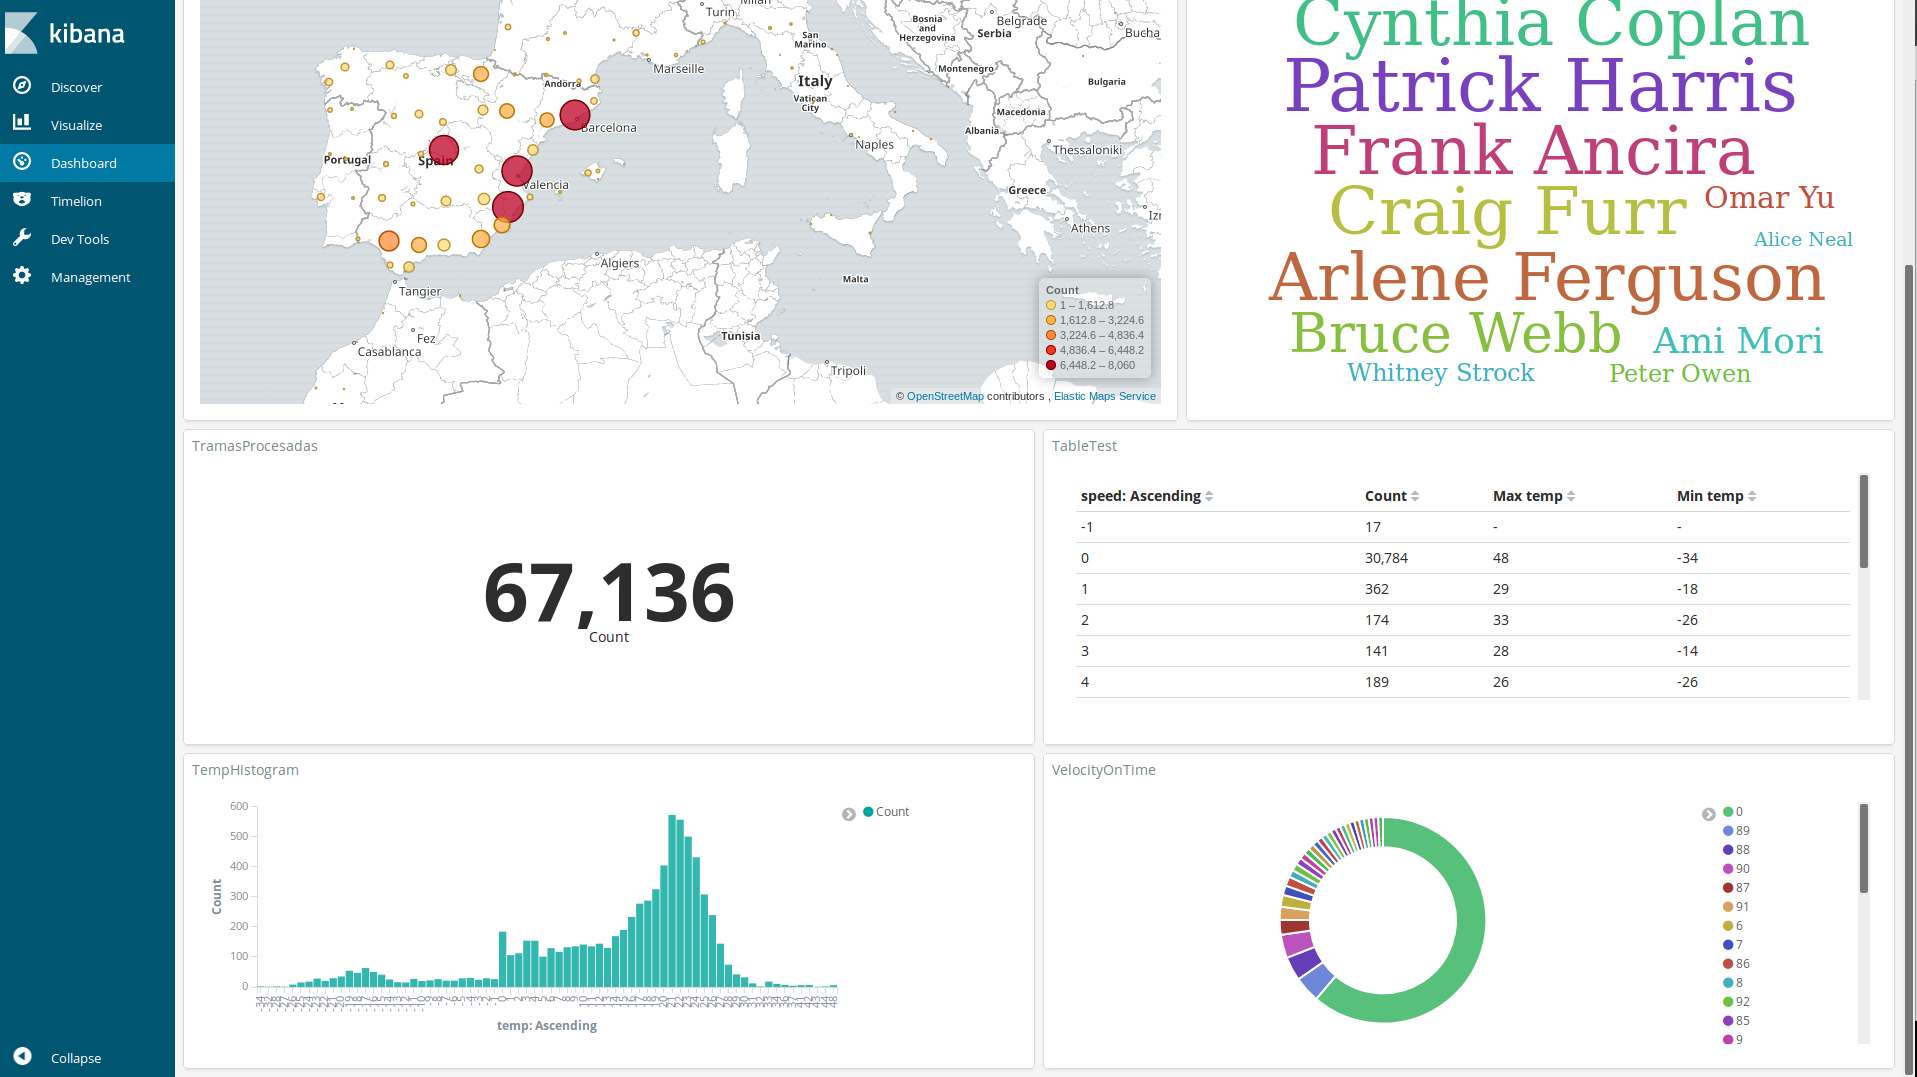
\includegraphics[width=150mm]{Imagenes/kibana1.png}}
		\subfigure{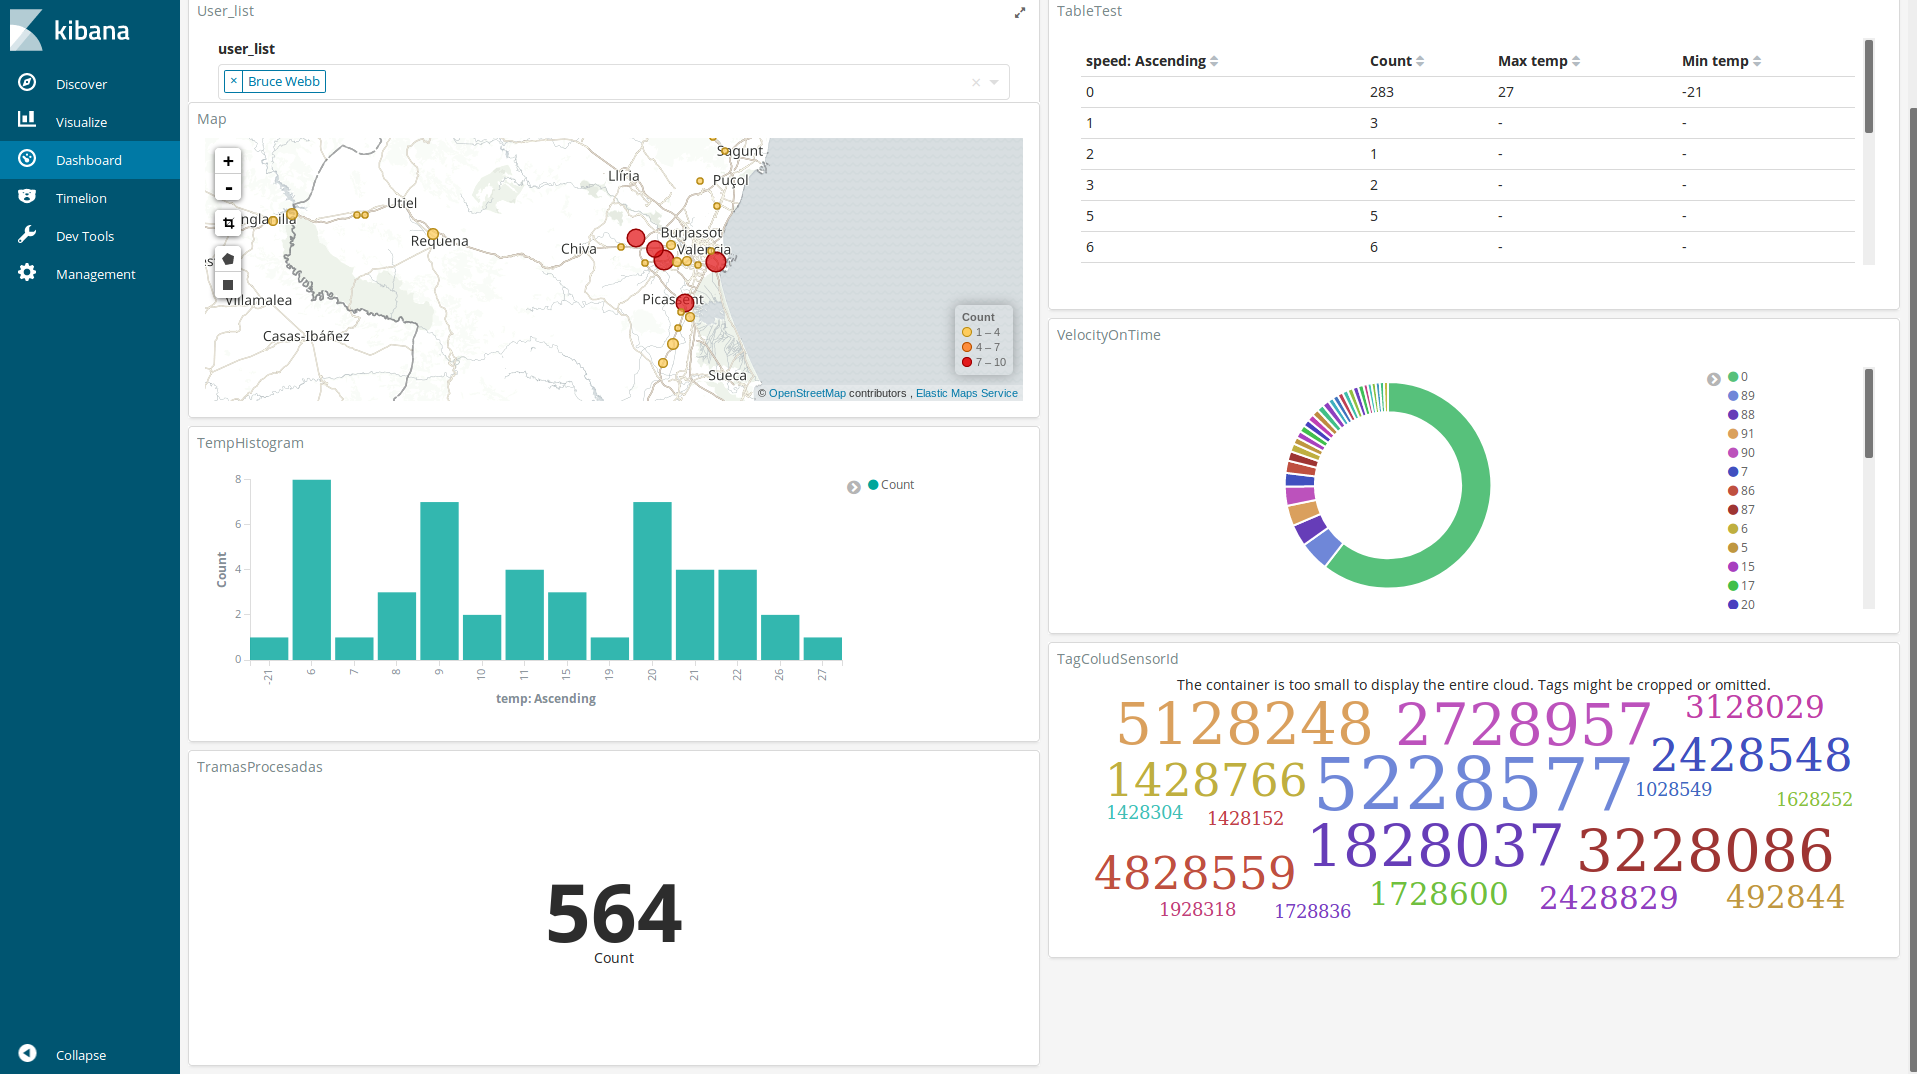
\includegraphics[width=150mm]{Imagenes/kibana2.png}}
%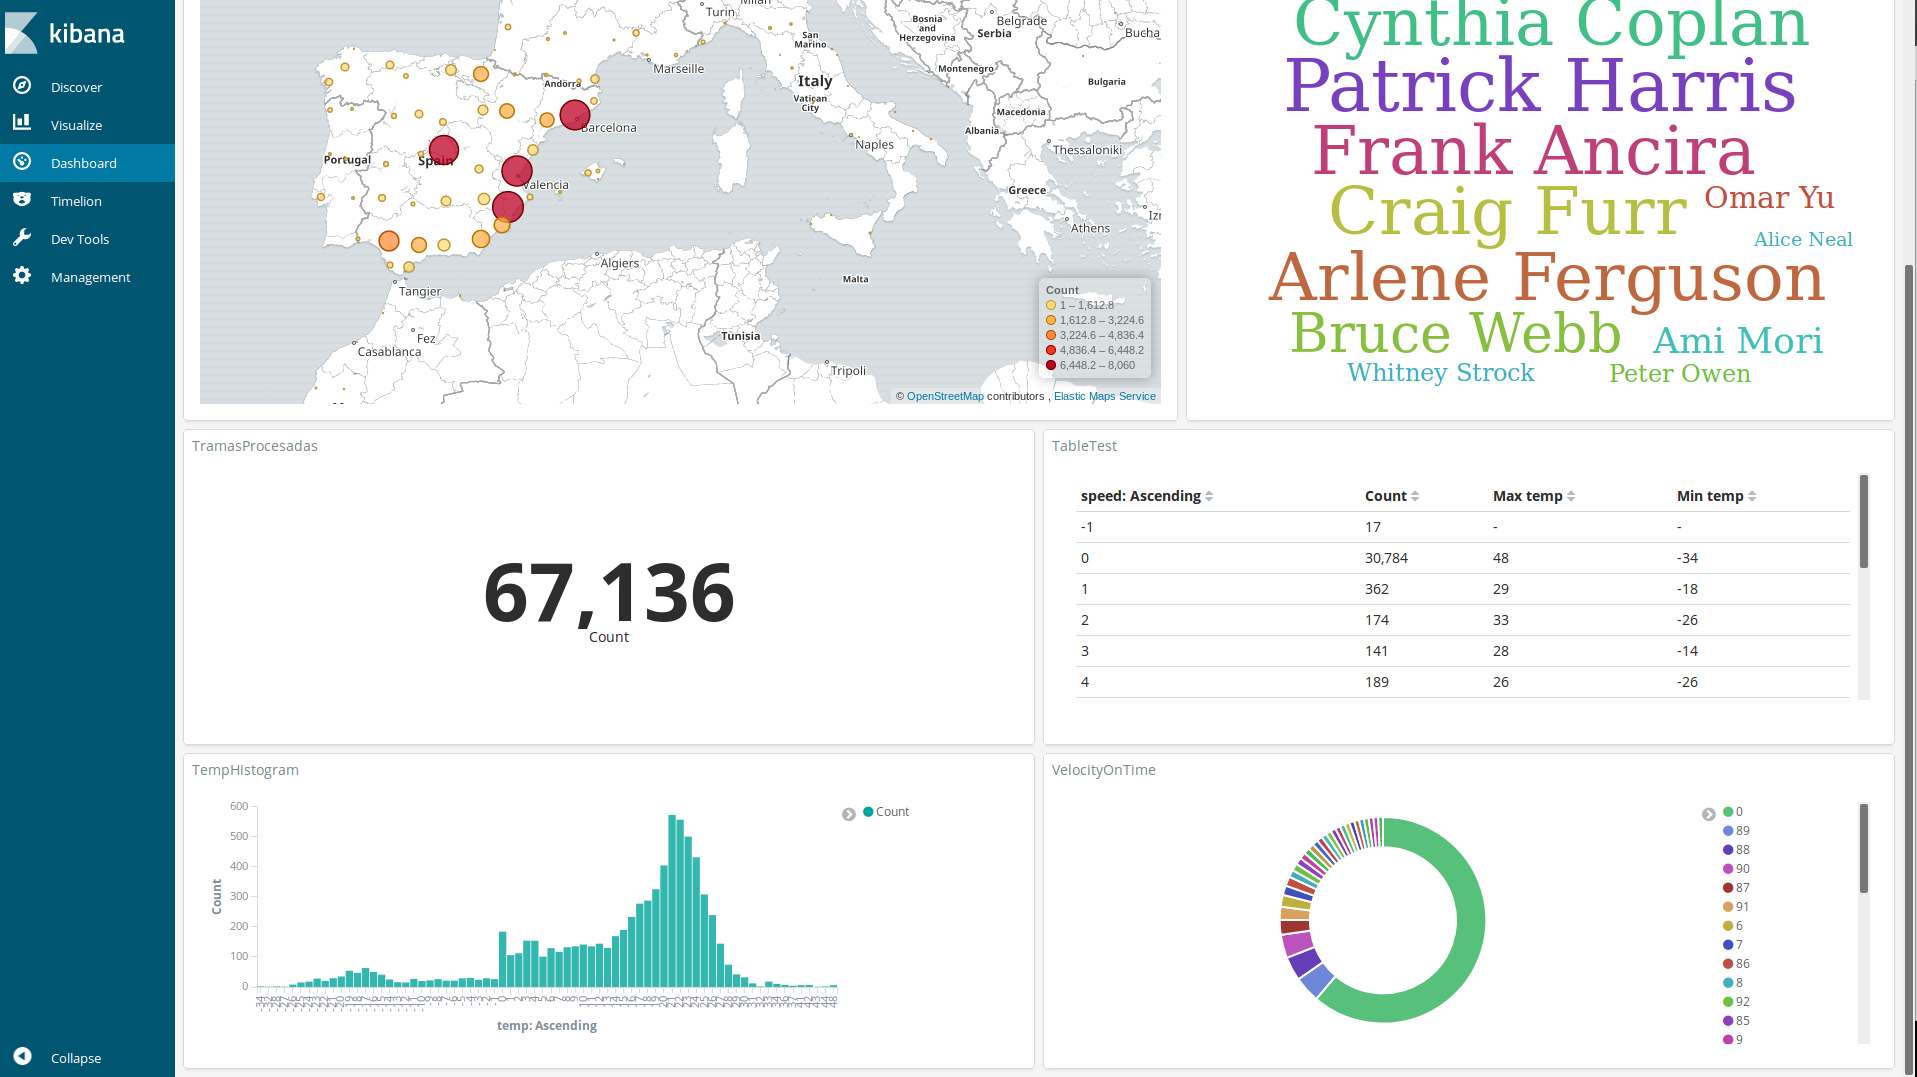
\includegraphics[scale=0.26]{Imagenes/kibana1.png}
\caption{Dashboards de Kibana}
\label{kibana1}
\end{figure}

%\begin{figure}[htp]
%\centering
%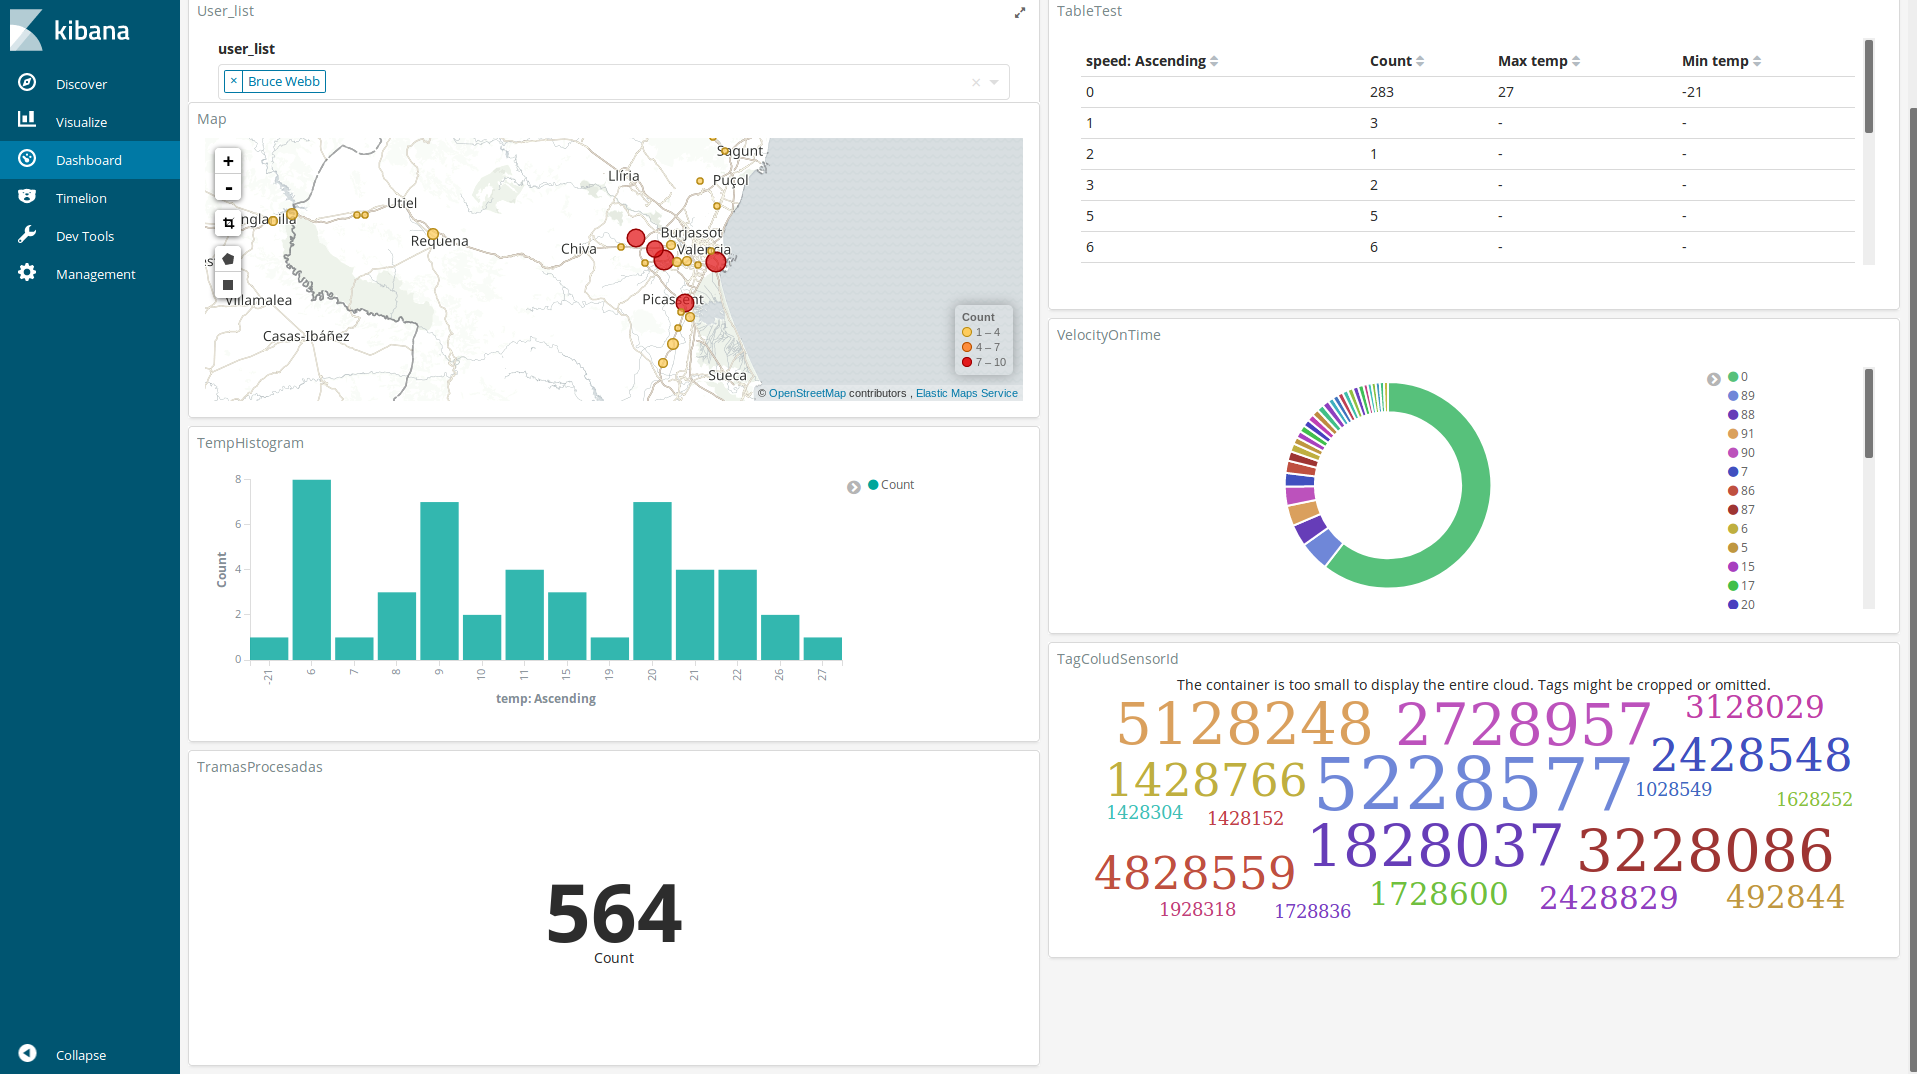
\includegraphics[scale=0.26]{Imagenes/kibana2.png}
%\caption{Dashboard de Kibana}
%\label{kibana2}
%\end{figure}
